% STRESS-Test — working draft v0.3 (not a released preprint)
% Build: pdflatex main && bibtex main && pdflatex main && pdflatex main
% (or upload the paper/ folder to Overleaf)
% Reported numbers are synchronized with the generated artifacts in results/.

\documentclass[11pt]{article}
\usepackage[T1]{fontenc}
\usepackage[utf8]{inputenc}
\usepackage[margin=1in]{geometry}
\usepackage{amsmath,amssymb}
\usepackage{booktabs}
\usepackage{graphicx}
\usepackage{microtype}
\usepackage{placeins}
\usepackage[numbers,sort&compress]{natbib}
\usepackage[colorlinks=true,citecolor=blue,linkcolor=blue,urlcolor=blue]{hyperref}
\usepackage{xcolor}
\hypersetup{
  pdftitle={STRESS-Test: Measuring the Reliability of AI-Text Detectors Under Real-World Transformations},
  pdfauthor={Mohammad Arifur Rahman},
  pdfsubject={Robust evaluation of AI-text detectors},
  pdfkeywords={AI-text detection, robustness, false-positive rate, trustworthy NLP}
}
\emergencystretch=2em
\newcommand{\qaes}{\textsc{qaes}}
\newcommand{\stresstest}{STRESS-Test}

\title{\stresstest: Measuring the Reliability of AI-Text Detectors\\
Under Real-World Transformations}

\author{Mohammad Arifur Rahman\\
\texttt{rahman.arif.cse@gmail.com}\\
\small Code and data: \url{https://github.com/razon1494/stress-test}}

\date{}

\begin{document}
\maketitle

\begin{quote}
\small\textbf{Draft status.} This is an active, pre-submission manuscript.
Reported results are preliminary: semantic-preservation thresholds have not yet
received the planned human validation, and the current calibration sensitivity
analyses do not use a fully independent calibration set.
\end{quote}

\begin{abstract}
Detectors of AI-generated text are deployed in classrooms, newsrooms, and hiring
pipelines on the strength of a single number: accuracy on clean text. We argue
this number measures the wrong thing, and present \stresstest, an evaluation
framework that measures detector \emph{reliability}: behaviour under realistic
transformations, at deployment operating points, symmetrically for both classes.
We formalize transformations as label-preserving metamorphic relations, freeze
each detector's threshold once at 1\% FPR on clean human text, and evaluate
seven detector families across fourteen conditions (clean plus thirteen
transformations), including composed
``laundering'' pipelines, and---critically---transformations applied to
\emph{human} text, including more than 2{,}200 essays by non-native English
writers across ten learner regions and four proficiency bands. Our preliminary
findings: (1) headline
accuracy and reliability rank detectors in nearly opposite orders---the
strongest clean-text detectors (97--98\% TPR) lose half or more of their
detection rate under a depth-2 paraphrase--translate pipeline, while a simple
case perturbation drives the GPT-2 perplexity detector from 93.1\% to 0.4\%
TPR; (2) evaluating attacked human text with threshold-free metrics,
as prior benchmarks do, hides a false-accusation problem: at frozen deployed
thresholds, false-positive rates change unevenly across writing registers and
writer groups, reaching double digits for both learner and native comparison
groups; related shifts also appear under gold or professional human editing,
not only model-generated editing; and (3) native status alone does not explain
the pattern: on topic-controlled prompt essays, \emph{native} writers are
flagged most. This is consistent with, but does not by itself establish, a
register/predictability account. We release the implementation, data recipes,
generated summaries, and an explicit validation roadmap.
\end{abstract}

\section{Introduction}

% Para 1: stakes — detectors are load-bearing infrastructure
Text-provenance detectors now gate consequential decisions: academic-integrity
referrals, content moderation, hiring screens. Commercial and open-source
detectors often advertise accuracies above 99\%, and benchmark summaries
commonly emphasize performance on clean machine text
\citep{dugan2024raid,li2024mage,wang2024m4gt}.

% Para 2: the gap — what existing evaluations measure vs what deployment needs
Deployment looks different. Text reaching a detector has typically passed
through tools---paraphrasers, translators, grammar checkers---or through a
human editor. Human-written inputs are equally consequential: an error is a
false accusation with real social
cost \citep{liang2023gpt}. Existing benchmarks address fragments of this
picture: RAID \citep{dugan2024raid} applies eleven adversarial attacks, but
one at a time and only to machine text; DetectRL \citep{wu2024detectrl}
perturbs human text but evaluates with threshold-free AUROC, concluding that
attacks on human text are ``minimal'' in impact or even helpful. We show this
conclusion can depend on the metric: AUROC cannot localize false-accusation
drift at a selected operating point, and our preliminary fixed-threshold
analysis reveals movement hidden by the ranking summary.

% Para 3: what we do
\stresstest{} evaluates \emph{reliability}, defined by four commitments:
(i)~\textbf{metamorphic evaluation}: every transformation is a
label-preserving metamorphic relation, so detector reliability is the
violation rate of these relations, and transformations compose into realistic
pipelines; (ii)~\textbf{threshold transfer}: thresholds are calibrated once,
at 1\% FPR on clean human text, and never re-tuned per condition;
(iii)~\textbf{symmetry}: every transformation is applied to human text too,
and false-accusation rates are first-class metrics, stratified by writer
proficiency (CEFR bands) and first-language background (ten countries);
(iv)~\textbf{quality control}: an ``evasion'' only counts if the transformed
text preserves meaning (quality-adjusted evasion, \qaes).

% Para 4: contributions list
\noindent Our contributions:
\begin{enumerate}
  \item A reliability evaluation framework covering seven detector families
        and fourteen evaluation conditions, including
        composed pipelines and \emph{gold human editing}, with
        document-clustered bootstrap inference throughout (\S\ref{sec:framework}).
  \item A re-examination of the ``attacks on human text are harmless'' claim
        \citep{wu2024detectrl}: at frozen thresholds, benign transformations
        can move false-accusation rates several-fold, with heterogeneous
        patterns across writing groups (\S\ref{sec:fairness}).
  \item Evidence that false-accusation patterns vary with writing register:
        non-native TOEFL-style writers and native writers of formulaic prompt
        essays can both be flagged at elevated rates. We evaluate a
        predictability-based account without treating it as causal
        (\S\ref{sec:register}).
  \item A hardness-aware analysis showing that example difficulty is
        detector-mechanism-relative: a difficulty score predictive for
        likelihood-based detectors anti-predicts for surface-feature
        classifiers (\S\ref{sec:hardness}).
  \item An auditable, consumer-GPU-scale implementation using open-weight
        models, deterministic document splits, data recipes, generated summary
        artifacts, and CI-tested research logic.
\end{enumerate}

\section{Related Work}
\label{sec:related}

\paragraph{Benchmarks.} RAID \citep{dugan2024raid} is the largest detection
benchmark (6.2M generations; 11 attacks applied singly to machine text;
per-domain thresholds at fixed 5\% FPR). DetectRL \citep{wu2024detectrl}
attacks human text (89.6k attacked human samples) but reports only AUROC/F1.
MAGE \citep{li2024mage} and M4GT-Bench \citep{wang2024m4gt} cover
generator/domain/language shift without a transformation axis. To our
knowledge, no single benchmark jointly evaluates composed transformations,
quality-conditioned evasion, hardness-stratified performance, and
false-accusation drift at deployed thresholds.

\paragraph{Attacks.} DIPPER \citep{krishna2023paraphrasing} showed paraphrase
evades detectors (DetectGPT $70.3\%\!\to\!4.6\%$ at 1\% FPR---the operating
point we adopt); \citet{sadasivan2023can} introduced recursive paraphrasing
and a TV-distance impossibility bound.\footnote{Their subtitle, ``Stress
Testing AI Text Detectors Under Various Attacks,'' predates our framework
name; the overlap is coincidental and the scopes differ---they stress-test
with attacks on machine text, we evaluate reliability symmetrically across
both classes. Our acronym expands to Semantic-preserving Transformations for
Robust Evaluation of Synthetic-text Screening.} Both measure attack-side quality as
aggregate tradeoffs; neither conditions per-example success on
embedding-filtered semantic preservation, and neither examines benign transformations of human
text.

\paragraph{Fairness.} \citet{liang2023gpt} found commercial detectors flag
61.2\% of non-native TOEFL essays on \emph{clean} text and that vocabulary
enhancement halves this. The interaction of this bias with text
transformations---the deployment-relevant question, since learner text is
disproportionately likely to pass through grammar tools---was previously
unmeasured.

\section{The \stresstest{} Framework}
\label{sec:framework}

\subsection{Transformations as metamorphic relations}
A transformation $t$ is admissible iff it preserves the gold provenance label:
$y(t(x)) = y(x)$. This is the invariant that licenses (a) composition---chains
$t_k \circ \cdots \circ t_1$ remain admissible---and (b) symmetric evaluation
on human text. We evaluate 14 conditions (clean plus 13 transformed conditions)
in 6 families: character/token
perturbations (homoglyph, zero-width, casing, typos, whitespace, contraction
expansion), paraphrase (T5), round-trip translation (EN$\to$FR$\to$EN),
model-based grammar correction \citep{raheja2023coedit}, \emph{gold human
editing} (real annotator corrections from W\&I+LOCNESS \citep{bryant2019bea}
and professional edits from ICNALE-EE \citep{ishikawa2023icnale}), and named
composed pipelines (e.g., \texttt{launder\_lite} = paraphrase
$\circ$ translation; \texttt{esl\_student} = translation $\circ$ grammar
correction).

\subsection{Threshold-transfer protocol}
For detector $d$ with score function $s_d$ (higher = more machine-like), the
threshold $\tau_d$ is the $(1-\alpha)$-quantile of a clean human calibration
pool with $\alpha = 0.01$, then frozen: every transformed condition, both
classes, is evaluated at $\tau_d$. In the current result set, however, the
calibration pool is drawn from the clean human portion of the evaluation data
(either pooled or per-domain), rather than an independent calibration split.
We therefore treat these operating-point results as sensitivity analyses; the
final protocol will reserve calibration documents before any test analysis.
Trainable detectors use clean training records only and are split by source
document. The fairness corpora are held out from detector fitting, but they
participate in the current clean calibration sensitivity analysis.

\subsection{Metrics}
Let $A(d,t)$ denote detector $d$'s TPR at threshold $\tau_d$ under condition
$t$, with $t{=}0$ denoting clean text. We report Robustness Score (RS),
Transformation Stability (TS), Worst-Case Performance (WCP), False-Accusation
Rate (FAR), Quality-Adjusted Evasion (\qaes), and Hardness Collapse Index (HCI):
\begin{align*}
\mathrm{RS}(d)   &= \frac{1}{|T|}\sum_{t \in T}\frac{A(d,t)}{A(d,0)}, \\
\mathrm{TS}(d)   &= 1-\mathrm{CV}_{t \in T}[A(d,t)], \\
\mathrm{WCP}(d)  &= \min_{t \in \text{pipelines}} A(d,t), \\
\mathrm{FAR}(d,t)&= \Pr\!\left[s_d(t(x))>\tau_d \mid y(x)=\mathrm{human}\right], \\
\qaes(d,t)       &= \Pr\!\left[\mathrm{evade} \mid
  \mathrm{sim}(x,t(x))\geq0.85\right], \\
\mathrm{HCI}(d)  &= \frac{A_{Q_1}-A_{Q_5}}{A_{Q_1}}.
\end{align*}
WCP is restricted to quality-valid named pipelines. QAES uses embedding
similarity \citep{reimers2019sentencebert}; its cutoff remains pending human
validation (\S\ref{sec:limitations}). HCI uses quintiles of a five-signal
hardness score fit with a leave-one-out detector committee
(\S\ref{sec:hardness}). All intervals are 95\% document-clustered bootstrap
CIs; detector comparisons use paired sign-flip permutation tests with Holm
correction.

\section{Experimental Setup}
\label{sec:setup}

\paragraph{Data.} Paired human/ChatGPT answers from HC3 \citep{guo2023hc3}
(1,361 pairs after length filtering, 5 domains) supply the machine-detection
core. Fairness corpora (all human, all held out from training):
\citet{liang2023gpt}'s public release (91 non-native TOEFL essays, 158 native
essays), W\&I+LOCNESS \citep{bryant2019bea} (CEFR bands A/B/C + native, with
gold corrections), and ICNALE \citep{ishikawa2023icnale} Written Essays
(10 countries + 400 native reference, topic-controlled) and Edited Essays
(655 original/professionally-edited pairs). Total: 5,294 records, 3,932
documents. Splits are document-level and hash-deterministic.

\paragraph{Detectors.} Seven families: TF-IDF + logistic regression;
stylometric features + GBM (GPTZero-style); GPT-2 perplexity; Fast-DetectGPT
(analytic) \citep{bao2024fastdetectgpt}; Binoculars \citep{hans2024binoculars}
(\emph{lite}: GPT-2/DistilGPT-2 observer--performer pair; deviation from the
original Falcon-7B pair is a stated limitation); the OpenAI RoBERTa GPT-2
detector \citep{solaiman2019release}; and our own DeBERTa-v3-base
\citep{he2023debertav3} fine-tuned on the HC3 train split (3 epochs, bf16,
single seed, single RTX 4050).

\section{Results}
\label{sec:results}

\subsection{Reliability inverts the leaderboard}
\label{sec:inversion}

Table~\ref{tab:leaderboard} shows the reliability cards under per-domain
calibration (one threshold per detector per domain; every detector's realized
clean FPR is 0.7--0.8\%, so rows are directly comparable). Ranked by clean
TPR, Fast-DetectGPT leads (97.7\%); ranked by worst-case pipeline performance
the ranking inverts: the supervised DeBERTa fine-tune retains 78.7\% under the
worst pipeline while the two strongest clean-text detectors retain 44--47\%.
TF-IDF and the stylometric baseline have the highest robustness scores
(0.96/0.92): the transformations that defeat likelihood-based detectors barely
move them---at the price of far lower clean detection.

\begin{table}[t]
\centering
\small
\begin{tabular}{lccccc}
\toprule
Detector & Clean TPR & RS & WCP & FAR gram.\ & FAR edit \\
\midrule
Fast-DetectGPT        & \textbf{97.7\%} & 0.73 & 46.7\% & 2.6\% & 3.4\% \\
Binoculars-lite       & 96.9\% & 0.63 & 44.0\% & 4.1\% & 7.4\% \\
DeBERTa-v3 (ours, ft) & 93.1\% & 0.83 & \textbf{78.7\%} & 4.0\% & 8.0\% \\
Perplexity (GPT-2)    & 93.1\% & 0.64 & 62.0\% & 5.7\% & 6.4\% \\
RoBERTa (OpenAI)      & 85.9\% & 0.55 & 53.3\% & \textbf{6.0\%} & 6.7\% \\
TF-IDF + LR           & 79.4\% & \textbf{0.96} & 63.3\% & 1.9\% & 1.1\% \\
Stylometric GBM       & 55.7\% & 0.92 & 50.7\% & 0.8\% & 1.2\% \\
\bottomrule
\end{tabular}
\caption{Reliability cards, per-domain calibration at target 1\% FPR (realized
clean FPR 0.7--0.8\% for every detector). WCP = minimum TPR over named
realistic pipelines (worst is \texttt{launder\_lite} for all). FAR columns:
false-positive rate on grammar-corrected and gold-human-edited human text at
the frozen thresholds. These thresholds are estimated from the same clean
domain slices, so the table is a calibration sensitivity analysis rather than
an independent test estimate.}
\label{tab:leaderboard}
\end{table}

\paragraph{Mechanism asymmetry.} Character-level noise that any normalizer
would remove is catastrophic for likelihood-based detectors: swapping the case
of $\sim$2\% of characters drives GPT-2 perplexity from 93.1\% to 0.4\% TPR;
zero-width spaces reduce it to 5.0\%, and homoglyph substitution to 17.2\%.
TF-IDF is essentially unchanged by those perturbations. RoBERTa falls to
0--0.8\% on the same three conditions, whereas DeBERTa is more robust to case
and homoglyph changes but falls to 1.1\% under zero-width insertion. Conversely,
semantic transforms leave the DeBERTa fine-tune near its clean rate (92.4\%
under paraphrase), though in-domain training caution applies
(\S\ref{sec:limitations}). \emph{The vulnerabilities are strongly
mechanism-dependent.} The repository includes normalization utilities, but a
full detector-level normalization ablation has not yet been reported.

\subsection{Threshold-free metrics can hide false-accusation movement}
\label{sec:fairness}

DetectRL \citep{wu2024detectrl} reports that perturbing human text
\emph{helps} detection (+10.2 AUROC on average) and concludes such attacks are
benign. At a frozen threshold, however, ranking metrics can hide movement in
false-accusation rates. Table~\ref{tab:cefr} shows that grammar correction and
gold human editing change FAR unevenly across detectors and writing groups.
The current fairness table uses one pooled threshold per detector; because that
threshold is estimated from the clean evaluation pool, the values are
exploratory rather than independent test estimates.

\begin{table}[t]
\centering
\small
\begin{tabular}{llcccc}
\toprule
Detector & Condition & CEFR A & CEFR B & CEFR C & Native \\
\midrule
Perplexity & clean             & 0.0\% & 1.0\% & 0.7\% & 7.3\% \\
Perplexity & grammar-corr.     & 1.0\% & 3.8\% & 1.3\% & 11.3\% \\
Perplexity & \emph{human edit} & 1.6\% & 0.7\% & 0.0\% & 0.0\% \\
RoBERTa    & clean             & 0.7\% & 0.8\% & 0.0\% & 6.0\% \\
RoBERTa    & grammar-corr.     & 6.8\% & 4.7\% & 3.4\% & \textbf{12.7\%} \\
RoBERTa    & \emph{human edit} & 1.6\% & 1.3\% & 2.7\% & 2.0\% \\
DeBERTa (ours) & grammar-corr. & 0.7\% & 4.1\% & 2.7\% & 8.0\% \\
Binoculars-lite & \emph{human edit} & 7.8\% & 6.7\% & \textbf{8.1\%} & 2.0\% \\
\bottomrule
\end{tabular}
\caption{False-accusation rate by CEFR proficiency band (W\&I+LOCNESS).
Clean/grammar-corrected rows contain $n=295/983/149/150$ records for
A/B/C/native; human-edit rows contain $n=128/150/149/50$.
``Human edit'' applies each essay's gold annotator corrections---no model
involved. Values are synchronized with \texttt{results/FAIRNESS.md}.}
\label{tab:cefr}
\end{table}

Three aspects of Table~\ref{tab:cefr} matter. First, gold human corrections can
also move FAR, so the phenomenon is not limited to CoEdIT outputs. Second, the
pattern is neither monotonic in proficiency nor confined to non-native writers;
the native comparison group has the largest grammar-corrected FAR for both
perplexity and RoBERTa. Third, the shape is detector-specific: Binoculars rises
under gold editing for all learner bands, while other detectors move in
different directions. Region-level ICNALE slices are similarly heterogeneous:
Japanese-L1 essays reach 9.4\%/11.7\% under perplexity/RoBERTa, but other learner
cells range from zero to 13.4\%. These descriptive cells require uncertainty
estimates and a confirmatory protocol before strong group-level conclusions.

\subsection{Register and predictability complicate native-status comparisons}
\label{sec:register}

On ICNALE's topic-controlled opinion essays the pattern changes:
native-speaker reference essays (ENS) are flagged \emph{most} (RoBERTa:
9\%$\to$19\% under grammar correction; perplexity: 11\%$\to$17\%), exceeding
every learner group in the same corpus. Figure~\ref{fig:register} suggests one
possible explanation:
by median GPT-2 negative log-likelihood, ICNALE's \emph{native} prompt essays
(2.81) sit closer to ChatGPT text (2.18) than any learner group does---closer
even than the non-native TOEFL essays (3.11)---while open-register human
writing is furthest (3.59). This pattern is consistent with
\citet{liang2023gpt}'s perplexity-mediation evidence and motivates a register
account: both limited-vocabulary learner writing and fluent native prose written
to a short, formulaic prompt can be statistically predictable. The present
analysis is descriptive, however; it does not isolate register from corpus,
prompt, or other population differences.

\begin{figure}[t]
\centering
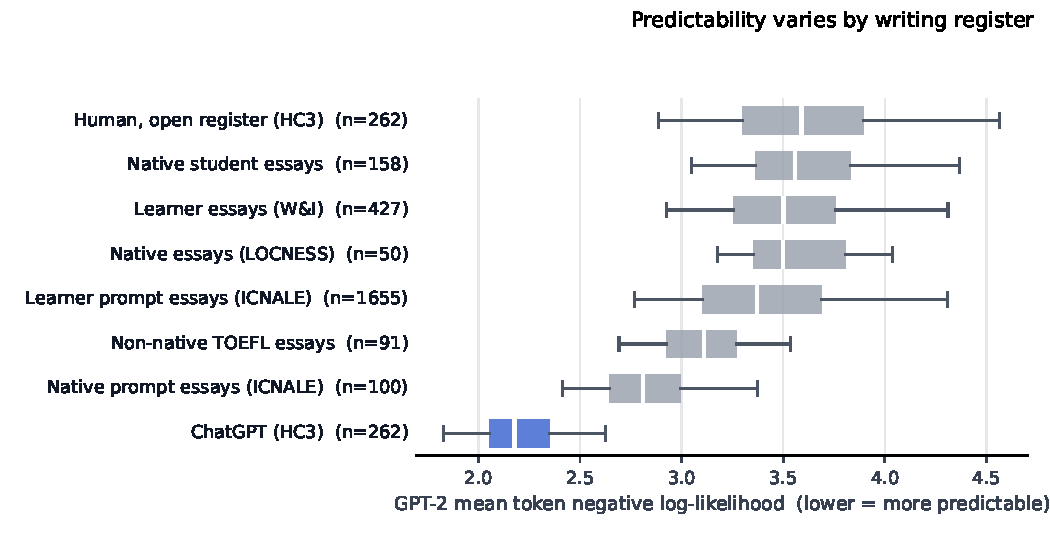
\includegraphics[width=0.96\linewidth]{figures/perplexity_by_corpus.pdf}
\caption{GPT-2 mean token negative log-likelihood by corpus group (boxes:
IQR; whiskers: 5th--95th percentile). In these descriptive samples, native
writers of topic-controlled prompt essays have lower median NLL than
non-native TOEFL writers. Corpus and register are confounded, so this figure
does not establish a causal mediation effect.}
\label{fig:register}
\end{figure}
\FloatBarrier

\subsection{Quality-adjusted evasion and composition}
\label{sec:qaes}

Composed pipelines are the worst case for every detector
(Table~\ref{tab:leaderboard}), but composition also destroys meaning: only
82\% of depth-2 \texttt{launder\_lite} outputs retain embedding similarity
$\geq 0.85$ to the original, against 94--96\% for single transforms, and
\qaes{} discounts evasion accordingly (e.g., perplexity under
\texttt{launder\_lite}: raw evasion 70.0\% vs.\ \qaes{} 67.5\%). The
correction is modest on our conditions---by design, since our transforms
target meaning preservation---but the machinery matters for attack papers
whose raw success rates conflate evading the detector with destroying the
text. The 0.85 similarity threshold is provisional pending the human
validation round (600 stratified pairs, 3 annotators, 200-pair overlap for
Krippendorff's $\alpha$; materials released with the benchmark).

\subsection{Hardness is detector-relative}
\label{sec:hardness}

We score per-example difficulty with five signals (perplexity closeness,
readability normality, lexical diversity \citep{mccarthy2010mtld}, semantic
consistency under paraphrase, leave-one-out committee margin), fit on a
transformed condition and frozen. The resulting HCI is positive and monotone
for likelihood-based detectors (Binoculars: 0.15; accuracy falls
94\%$\to$80\% from the easiest to hardest quintile under paraphrase) but
\emph{negative} for
surface classifiers (RoBERTa $-0.04$; TF-IDF $-0.02$): examples our score
calls hard are where those detectors do \emph{better}. Difficulty, as commonly
operationalized through likelihood-adjacent signals, is not a property of the
text alone but of the text--detector pair; benchmarks assuming a universal
$H(x)$ implicitly favour the detector family their signals resemble.

\subsection{Calibration-pool sensitivity}
\label{sec:calibration}

Freezing FPR requires choosing \emph{whose} human text defines the threshold.
Under a single pooled threshold, moving the calibration pool from HC3-only to
one including learner and essay registers cut TF-IDF's clean TPR from 79.4\%
to 57.3\% and RoBERTa's from 78.6\% to 51.9\%, while Binoculars moved by
$<$1pp---surface classifiers are hostage to calibration-pool composition in a
way likelihood detectors are not. Per-domain calibration
(Table~\ref{tab:leaderboard}, following \citealp{dugan2024raid}) removes the
artifact: every detector then realizes 0.7--0.8\% clean FPR and recovers its
in-register TPR. Because each per-domain threshold is estimated from the same
clean domain slice used to report clean FPR, this is a sensitivity analysis,
not evidence of held-out deployment performance. The contrast motivates a
confirmatory run with separate, register-aware calibration data.

\section{Limitations}
\label{sec:limitations}

We state these plainly. (1) Machine text derives from HC3 (single generator
family, QA register); generator diversity (MAGE/RAID sources) is wired but
not yet run at scale. (2) The DeBERTa fine-tune's paraphrase robustness may
partly reflect in-domain training; the OOD-generator slice must gate any
general claim. (3) Binoculars-lite uses a small model pair, not the original
Falcon-7B pair. (4) Semantic preservation is embedding-scored; the human
validation round (planned, $\sim$600 stratified pairs, 3 annotators) has not
yet run, so \qaes{} thresholds are provisional. (5) Thresholds in the current
result set are estimated from clean human records in the evaluation pool; a
separate calibration split is required for final operating-point estimates.
(6) Single seed for the fine-tune; per-country fairness cells are $n \leq 180$
and the public slice table does not yet include confidence intervals.
(7) All experiments ran on one consumer GPU; scale is bounded accordingly.
(8) Licensed corpora, model weights, and per-example score caches are not
distributed in this repository; only code, data recipes, and generated summary
artifacts are committed.

\section{Conclusion}
Reliability, not clean accuracy alone, is the quantity deployment depends on,
and the two can rank detectors differently. Evaluated symmetrically at a fixed
threshold, benign transformations of human writing can produce
false-accusation movement that threshold-free evaluation cannot localize. The
present slices associate that movement with writing register and predictability,
but do not support causal claims about writer identity. We release the
\stresstest{} code, data recipes, generated summary artifacts, and validation
materials as a transparent foundation for the next confirmatory evaluation.

{\small
\bibliographystyle{plainnat}
\bibliography{references}
}

\end{document}
